\documentclass[10pt,a4paper]{article}
\usepackage[utf8]{inputenc}
\usepackage[english]{babel}
\usepackage[T1]{fontenc}
\usepackage{amsmath}
\usepackage{amsfonts}
\usepackage{amssymb}
\usepackage{graphicx}
\usepackage{listings}
\author{Milan Tepic, Ivan Antunovic, Jung A Yoon, Peter von Zameck Glyscinski}
\title{Assignment 2 Team 5}

\begin{document}
\maketitle

\section*{Task 1}
\subsection*{a)}
Lets assume we have a task set $\mathbb{T}= \left\{ \begin{array}{c}
											T_1=(4,1,4),\\
											T_2=(5,2,7),\\
											T_3=(20,3,20),\\
											T_4=(20,2,20),\\
											\end{array}\right.$
which has Utilization $U = \frac{1}{4} + \frac{2}{5} + \frac{3}{20} + \frac{2}{20} = \frac{18}{20} < 1$.
The hyperperiod of this task set would be $H= lcm(4, 5, 20) = 20$ and a Framesize $F=4$ would fullfill the 3 constraints:
\newline
$20 ~mod ~4 = 0$
\newline
$4 \geq max(1, 2, 3) = 3$
\newline
$8 - gcd(4, 4) = 4 \leq 4$
\newline
$8 - gcd(5, 4) = 7 \leq 7$
\newline
$8 - gcd(20, 4) = 4 \leq 20$
\newline
$8 - gcd(20, 4) = 4 \leq 20$
\newline 
But if we try to schedule the task set with frame size $F = 4$ we get no feasible scheduling like we can see in figure \ref{fig:1a}.

\begin{figure}[h]
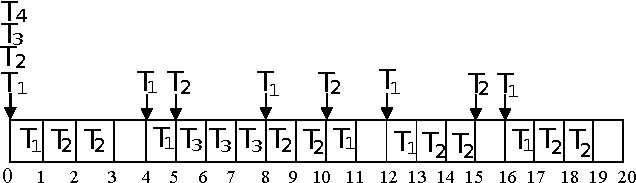
\includegraphics[width=\linewidth]{timing-diagram1a.pdf}
\caption{Task set $\mathbb{T}$ is not schedulable since $T_4$ is missing its deadline.} 
\label{fig:1a}
\end{figure}
\subsection*{b)}
\subsubsection*{i)}
Hyperperiod $H = lcm(20,24,30,32,28,27,35,21,42,36) = 30240$

\subsubsection*{ii)}
Possible frame sizes are
\newline
$F\in \{2, 3, 4, 5, 6, 7, 8, 9, 10, 12, 14, 15, 16, 18, 20, 21, 24, 27, 28, 30, 32, 35, 36, 40, 42, 45, 48, 54, 57,$
$60, 63, 70, 72, 80, 84, 90, 96, 105, 108, 112, 120, 126, 135, 140, 144, 160, 168, 180, 189, 210, 216, 224,$
$240, 252, 270, 280, 288, 315, 336, 360, 378, 420, 432, 480, 504, 540, 560, 630, 672, 720, 756, 840, 864,$
$945, 1008, 1080, 1120, 1260, 1440, 1512, 1680, 1890, 2016, 2160, 2520, 3024, 3360, 3780, 4320, 5040,$
$6048, 7560, 10080, 15120\}$
\newline
Which are 94 possibilities without taking into account the 1 and the 30240.

\subsubsection*{iii)}
Smallest frame size $F$ which satisfies the second constraint is $max(3, 2, 3, 3, 1, 1, 4, 1, 5, 4) = 5$

\subsubsection*{iv)}
\begin{equation}
2 * 12 - gcd(12, 20) = 24 - 2 = 22 > 20
\end{equation}
Not working for $F=12$

All Tasks are working for $F=10$ because $2*F$ is always smaller than $p_i$
\begin{equation}
2 * 10 - gcd(10, 20) = 20 - 10 = 10 \leq 20
\end{equation}


\subsubsection*{v)}
$\# of frames = \frac{hyperperiod ~H}{framesize ~F} = \frac{30240}{20} = 1512$ 

\subsection*{c)}

\begin{tabular}{| c | c | c || c | c | c |}
  \hline
  Task $i$ & $p_i$ & $e_i$ & 1st exec. & 2nd exec. & 3rd exec. \\
  \hline
  0 & 200 & 1 & 0 & 200 & 400 \\
  \hline
  1 & 200 & 2 & 1 & 201 & 401 \\
  \hline
  2 & 300 & 3 & 3 & 300 & 603 \\
  \hline
  3 & 300 & 4 & 6 & 303 & 606 \\
  \hline
  4 & 200 & 5 & 10 & 203 & 403 \\
  \hline
  5 & 600 & 6 & 15 & 615 & 1215 \\
  \hline
\end{tabular}

\subsection*{d)}
\begin{tabular}{| c | c | c | c |}
\hline
Frame \# & frame start & frame end & tasks \\
\hline
0 & 0 & 120 & 0,1,2,3,4,5 \\
\hline
1 & 120 & 240 & - \\
\hline
2 & 240 & 360 & 0, 1, 4 \\
\hline
3 & 360 & 480 & 2, 3 \\
\hline
4 & 480 & 600 & 0, 1, 4 \\
\hline
\end{tabular}
\end{document}